% Opcje klasy 'iithesis' opisane sa w komentarzach w pliku klasy. Za ich pomoca
% ustawia sie przede wszystkim jezyk i rodzaj (lic/inz/mgr) pracy, oraz czy na
% drugiej stronie pracy ma byc skladany wzor oswiadczenia o autorskim wykonaniu.
\documentclass[english,inz,shortabstract]{iithesis}

\usepackage[utf8]{inputenc}

%%%%% DANE DO STRONY TYTUŁOWEJ
% Niezaleznie od jezyka pracy wybranego w opcjach klasy, tytul i streszczenie
% pracy nalezy podac zarowno w jezyku polskim, jak i angielskim.
% Pamietaj o madrym (zgodnym z logicznym rozbiorem zdania oraz estetyka) recznym
% zlamaniu wierszy w temacie pracy, zwlaszcza tego w jezyku pracy. Uzyj do tego
% polecenia \fmlinebreak.
\polishtitle    {Aplikacja do zarządzania portfelami kryptowalut}
\englishtitle   {Application for cryptocurrency wallets management}
\polishabstract {
Kryptowaluty są praktycznym zastosowaniem technologii blockchain.
Do głównych operacji przeprowadzanych przez posiadaczy tych cyfrowych dóbr, należą:
zakładanie portfeli, śledzenie ilości środków oraz wykonywanie transakcji.
Celem tej pracy jest dostarczenie metody ich realizacji na różnych blockchainach.
Efektem końcowym jest napisany w Pythonie program, zintegrowany z Bitcoinem i Ethereum,
umożliwiający użytkownikom wykonywanie na nich operacji finansowych w ujednolicony sposób.
}
\englishabstract{
Cryptocurrencies are a practical application of the blockchain technology.
Crucial operations conducted by owners of such digital assets include:
creating wallets, tracking the amount of funds and making transactions.
This thesis aims to deliver a method of carrying them out on different blockchains.
The result is a program written in Python, integrated with Bitcoin and Ethereum,
allowing users to perform financial operations on them in an unified way.
}
% w pracach wielu autorow nazwiska mozna oddzielic poleceniem \and
\author         {Sławomir Górawski}
% w przypadku kilku promotorow, lub koniecznosci podania ich afiliacji, linie
% w ponizszym poleceniu mozna zlamac poleceniem \fmlinebreak
\advisor        {dr Leszek Grocholski}
%\date          {}                     % Data zlozenia pracy
% Dane do oswiadczenia o autorskim wykonaniu
%\transcriptnum {}                     % Numer indeksu
%\advisorgen    {dr. Jana Kowalskiego} % Nazwisko promotora w dopelniaczu
%%%%%

%%%%% WŁASNE DODATKOWE PAKIETY
%
%\usepackage{graphicx,listings,amsmath,amssymb,amsthm,amsfonts,tikz}
\usepackage{graphicx,bibentry}
%
%%%%% WŁASNE DEFINICJE I POLECENIA
%
%\theoremstyle{definition} \newtheorem{definition}{Definition}[chapter]
%\theoremstyle{remark} \newtheorem{remark}[definition]{Observation}
%\theoremstyle{plain} \newtheorem{theorem}[definition]{Theorem}
%\theoremstyle{plain} \newtheorem{lemma}[definition]{Lemma}
%\renewcommand \qedsymbol {\ensuremath{\square}}
% ...
%%%%%

\begin{document}

%%%%% POCZĄTEK ZASADNICZEGO TEKSTU PRACY

\chapter{Introduction}

Cryptocurrency is a digital asset designed to work as a medium of exchange,
history of which can be traced back to 2008, when Satoshi Nakamoto's
Bitcoin white paper was published \cite{bitcoin-white-paper}.
Since that time the blockchain technology
Bitcoin was based on has gained a significant popularity,
giving birth to a huge number of different projects.
Tha applications of it are various,
this thesis will be focused on the most widespread one -- cryptocurrency.

Since 2008 the technology has significantly evolved,
and with three distinct blockchain generations being distinguished \cite{blockchain-generations}
and over 2300 various cryptocurrencies available over the internet \cite{cryptocurrency-list},
it may seem challening to comprehend.
With such a vast array of different digital assets for the users to exchange,
wrapping one's head around them is likely a non-trivial task.

This project aims to provide a partial solution by creating
an application for cryptocurrency wallets management
-- an unified interface for performing common financial operations
across different blockchains.
Chosen for this purpose were Bitcoin and Ethereum \cite{ethereum-white-paper},
belonging respectively to first and second generation,
as popular choices among users \cite{currencies-popularity} which together should provide
a comprehensive overview of the technology as a whole.

\chapter{Description and analysis of the subject}

To decide on the best approach to the challenge,
first an analysis of desired properties and features of a solution
shall be conducted.
After that the technologies that the project will have to work with
will be looked into, with the goal to determine how are they similar,
and at the same time, how they differ.

\section{Definition of the goal}

To compile a list of features that ought to be demanded
from a crypto wallet management application,
we can compare it to services used by more traditional
internet banking.
As other applications of the blockchain technology,
for example smart contracts,
are out of this thesis' scope,
focus is to be on financial management.

The core functionality that the project cannot be considered complete without is to be:
\begin{itemize}
    \item creating cryptocurrency wallets,
    \item checking the amount of funds,
    \item making transfers.
\end{itemize}
All of the above should function in a similar way
from the end user's perspective
across all supported cryprocurrencies.

With these implemented an user should have sufficient control
over their crypto assets,
allowing him to participate in either personal or proffesional
financial operations over the cryptocurrency networks.

Some additional features, that would be convenient to have,
however will not be considered essential could be:
\begin{itemize}
    \item saving wallets' balance history,
    \item insight into value of the crypto assets (e.g. in US dollars),
    \item ability to import wallets used previously with other services.
\end{itemize}

The project should provide all this functionality
while remaining stable and portable,
prove resistant to predictable user errors
and ensure that managed assets' security will not be compromised.
The user experience ought to be simple,
and the interface should be clean and focused on the most important elements,
with function taking precedence over form.

\section{Technology overview}

The project will have to integrate with two blockchain generations:
first generation, represented by Bitcoin, the oldest and most known
cryptocurrency, and second generation, represented by Ethereum.
Although these cryptocurrencies have a lot in common
-- they both are based on blockchain, after all
-- they differ even in what they were to be.

Bitcoin was created as a peer-to-peer electronic cash system,
aiming to provide an alternative to traditional banking
-- performed through financial institutions
-- with a concept of a global,
distributed ledger of transactions,
secured from being mangled with by proof-of-work
in form of using computational power to mine blocks of transactions,
thus preventing them from being retroactively changed.

The premise of Ethereum was a bit different,
as it was focused more on distributed computation,
aiming to deliver what can be thought of as a decentralized computer,
with global state made of accounts containing information such as balance,
being secured by the blockchain technology.
The solution used currently for mining blocks is also proof-of-work,
although that is said to change in near future.

\subsection{Similarities}

Both technologies are interacted with through asymmetric cryptography
-- users are identified by their addresses and authorize operations
by signing data with their private keys.
In the core essence, a cryptocurrency wallet is all about its private key.
A public key is coupled with the private key,
and then an address is derived from the public key
as an additional layer of security.
This is true for both blockchains
-- even though the format of keys and addresses differs,
underlying principle remains the same.

\subsection{Differences}

As was hinted before, Ethereum accounts are stateful by nature,
Bitcoin ones, however, are not.
This difference is apparent when certain information needs to be
recovered from the blockchain.
It is often the case when it's saved as part of the Ethereum network's
global state and the extraction is straightforward.
Bitcoin is not based on a notion of any global state,
so in theory crawling an entire blochchain
might be required for reconstructing the current situation.

A good example of this is wallet balance
-- a part of the account state in Ethereum, easy to recover.
Bitcoin does not however deal with accounts directly,
it deals only with transactions;
so this quite basic piece of information might require
tracing all transactions somehow associated with a given wallet,
possibly many years into the history of Bitcoin.

\subsection{Conclusions}

Seamless integration of the project with both blockchains,
with details abstracted away under a shared interface
might prove a nontrivial task,
as there are quite substantial
differences in how these function.

However, the similarities between Bitcoin and Ethereum
make the same task seem sensible and worth the effort,
as for an end user dealing with cryptocurrencies,
both are in their essence just digital assets,
so providing an unified way to manage them
sounds like an useful idea.

\chapter{Comparison with other known solutions} \label{3}

Two applications that provide similar functionality
and can be compared with this project are Copay \cite{copay} and MyEtherWallet \cite{mew}.
Following sections will provide a brief overview of their features
and how the project tries to improve on them.

\section{Copay}

Copay is a popular application for Bitcoin wallets management.
It's an open source client created by BitPay Inc,
currently featuring hundreds of contributors.
By default, it utilizes Bitcore Wallet Service as its backend
for conntecting to the network, however it can be configured
to integrate with user's custom nodes.

\begin{figure}[ht]
    \centering
    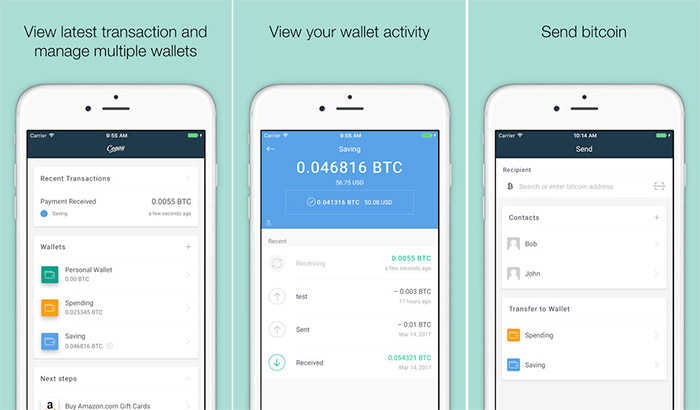
\includegraphics[width=0.7\textwidth]{assets/copay.jpg}
    \caption{Copay interface on a mobile device}
    \label{3:fig:copay}
\end{figure}

\newpage

The application itself is multi-platform, written in JavaScript \cite{javascript}.
On desktop operating systems, it runs on top of Electron \cite{electron}.
It allows for creating wallets, viewing balances and making transfers,
so all the operations considered essential in this thesis are covered.
However the supported currencies currently are Bitcoin and Bitcoin Cash,
which is a fork of Bitcoin -- so in essence just one type of blockchain.
Apparently, the goal here was quality support for few currencies.

The multi-platform nature of the application is quite problematic
on its desktop versions.
The interface is clearly designed mobile-first
and using it with keyboard and mouse is not comfortable.
The screens that the user interacts with display
very limited amounts of information at once,
and accessing some of the less obvious options
often requires traversing several views.
While this kind of design may work well if used on a mobile device,
it does not provide a good user experience for a desktop application.

An interesting fact about Copay is that it has quite recently been
a target of a rather sophisticated attack \cite{copay-attack},
which aimed to steal private keys of users, who possessed more than
100 bitcoins on their wallets.
That incident might have undermined users' trust
in security of the application.

\section{My Ether Wallet}

My Ether Wallet is a wallet management service for Ethereum
and some of the tokens available on its network.
The client is a single page application created in JavaScript
and available under the address \url{https://www.myetherwallet.com}.
The entire project received a design makeover recently,
however its new version does not seem to provide all of the features
available in the previous one yet, so the comparison will be done
in regard to the older version, which is still available at
\url{https://vintage.myetherwallet.com}.

\begin{figure}[ht]
    \centering
    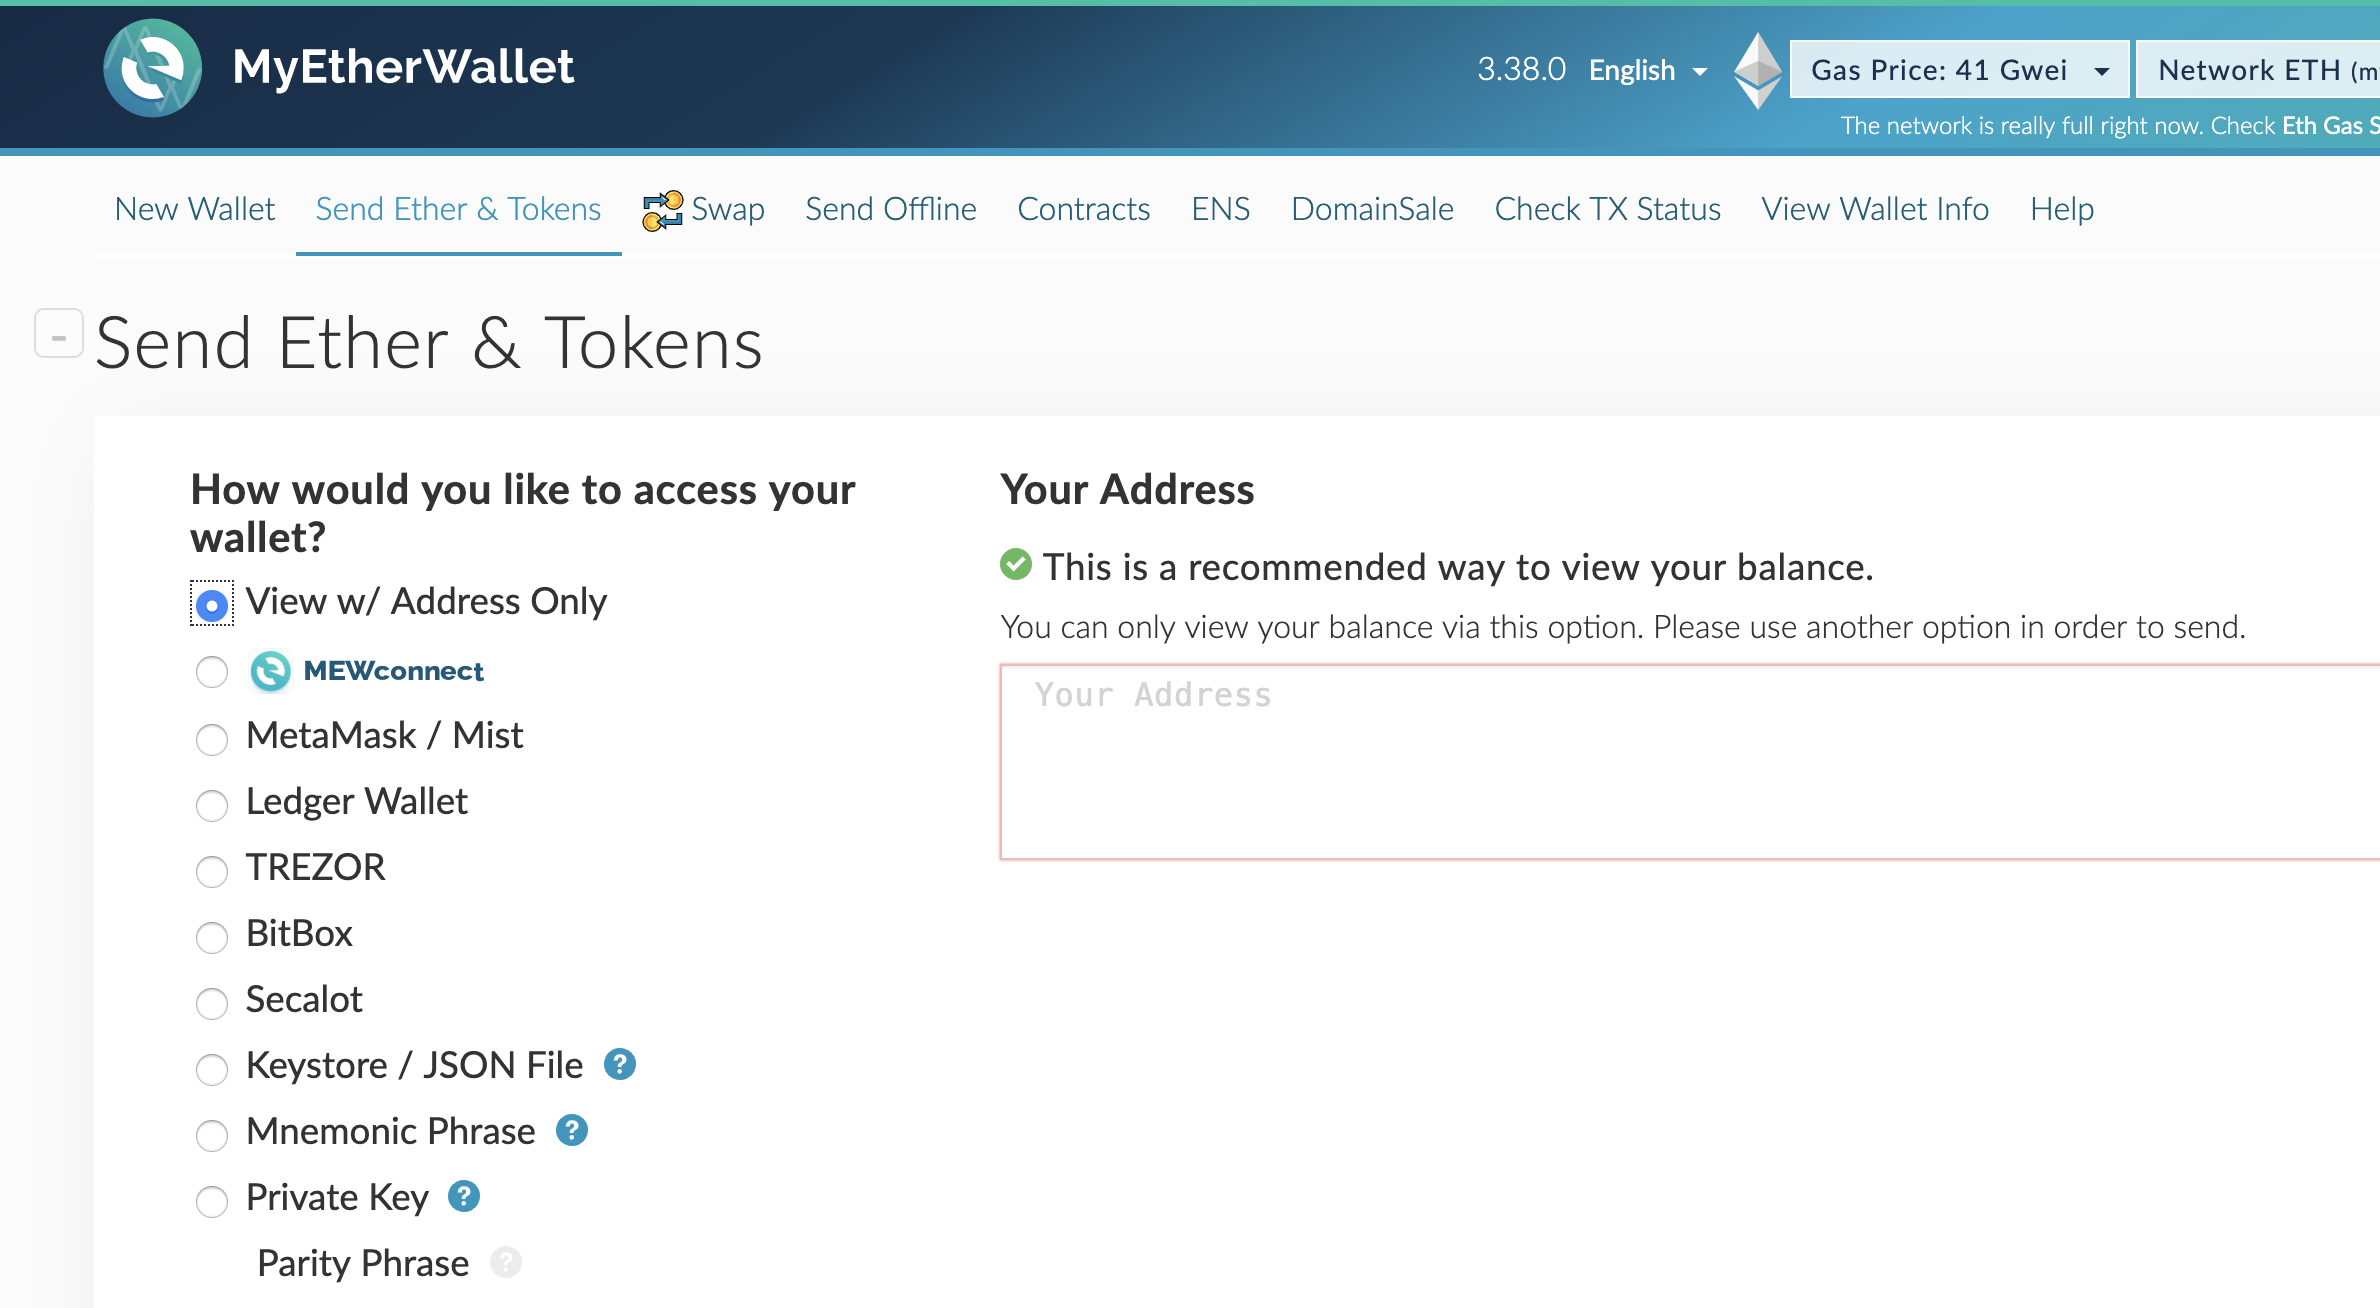
\includegraphics[width=0.7\textwidth]{assets/mew.png}
    \caption{My Ether Wallet website}
    \label{3:fig:mew}
\end{figure}

\newpage

The application is quite feature-rich and allows for connecting
with custom nodes and performing all the necessary operations.
A major advantage is that everything works out of the box
in browser, without the need of installing anything on user's device.

What can be disliked in this application is again the user interface,
although for different reasons than Copay's one.
While this one looks as if it was designed desktop-first, makes good use
of the entire screen and can be comfortably operated with a keyboard and a mouse,
it feels cluttered.
There are too many options displayed on a single screen,
and upon first access an alert with a rather invasive explanation
of how the website works is displayed,
and to make it not appear on user's device
they are forced to read through several screens.

Another major issue with the MyEtherWallet user experience
is that upon refreshing a page, the entire session is lost.
While it might be a good security choice in context of
accessing wallets by their private keys,
it provides a rather poor experience while viewing
wallet by its address.
Not only is the user forced to input it again,
they are also shown the intrusive alert described above
and have to deal with it as well.

\chapter{Description of applied solutions}

The entire project consists of two parts:
\begin{itemize}
    \item a library,
    which provides a unified interface for connecting to and performing operations on the blockchains,
    \item a web application using that library,
    which provides a convenient interface for the users and a couple of extra features.
\end{itemize}

Such separation makes it easy to potentially change the user interface, e.g. to a command line one,
while being able to preserve a convenient way of interacting with the blockchains.
It also allows for a better control over the project's dependencies,
-- where the library isn't cluttered with requirements of any web framework
-- and makes testing easier.
Core functionality of the library can be fully verified without being restricted by the user interface. Application tests, on the other hand, can have the library calls mocked out,
enabling them to be performed without access to the cryptocurrency testnets,
which makes setting up particular scenarios easier.

\section{Library}

The library is essentially a set of classes with an unified interface for typical wallet management operations, i.e.:
\begin{itemize}
    \item creating a new wallet or retrieving one,
    \item checking balance on a given wallet,
    \item sending money to other wallets of given currency,
\end{itemize}
which shall be explained in more detail below.

\subsection{Creating wallets}

This operation is performed nearly the same way on either blockchain.
First, a private key is either randomly generated, or recovered from a mnemonic phrase.
Next, a public key is retrieved from the private key, and then an address is derived from it.
The public key is not really relevant to the user,
as the address is used in its stead to provide an additional layer of security \cite{bitcoin-addresses}.
Expected format of these pieces of data may differ (e.g. it's hexadecimal in Ethereum),
but the underlying principle remains the same.
Overall, the private key, the address and a mnemonic phrase
allowing to easily recover this wallet later are returned.

A question may arise whether the mnemonic phrase is required, since a private key
already provides control over a wallet?
Essentially, it is not, and the information stored in it is equivalent,
however its format makes it easier for humans to remember,
than a key which is a long, seemingly random sequence of characters.

Theoretically, this whole procedure is independent from the blockchain,
as a wallet is just a combination of keys and can be generated offline.
In principle, that is the case, as it should be in a decentralized network.
However, there is a catch -- in the case of Bitcoin a wallet's address is imported by a node for indexing.
This will be explained in the following subsection.

\subsection{Checking balances}

Retrieving the amount of money available on a given address works a bit differently in the two networks.
The Ethereum accounts are stateful by nature, storing that information directly in themselves
-- all it takes to view it is a single remote procedure call to our node in the network.

In Bitcoin, however, this is not the case -- only transactions are stored in the blockchain,
balances are not. In order to determine how much money does one have at their disposal,
they would have to crawl the chain tracing the flow of money related to their address,
possibly many blocks in, even to the very beginning of Bitcoin.

In practice Bitcoin node implementations provide a solution for this,
indexing transactions related to given addresses,
which makes it possible to retrieve all unspent transactions outputs \cite{utxos} for an address
without crawling the blockchain every time.
Each of these UTXOs (Unspent Transaction Outputs) can be used to make a transfer,
which means that the balance of a wallet is a sum of their amounts.

\newpage

\subsection{Making transfers}

The last operation is rather easy in the case of Ethereum,
where a transaction is constructed by specifying sender, recipient, amount
and the appropriate gas price.
The latter serves (in a rather indirect way) as fee for block miners
and can be inferred from network activity using a built-in procedure of the node.
There is also \textit{nonce}, which is like an account's transcation counter
-- its appropriate value is just a number of our unconfirmed transactions in the network.

When making a transfer to more than one recipient (let us say there are $n$),
$n$ transactions are created, with \textit{nonce} iteratively incremented for each one.
The downside of this simple approach is that the gas price must be provided separately,
so we end up paying $n$ miner fees for all of the transactions.

As was described earlier, Bitcoin deals with transfers, not with accounts,
and this results in a more complex way of creating a transaction.
Some of our unspent transaction outputs must be selected to serve as input to the new transactions,
and they must be spent entirely.
If their total value is too high,
our own address is added as one of the recipients to receive change.
After that step we end up with a transaction object with some inputs
-- worth in total $x$ BTC
-- and recipients (including us) to receive in total $y$ BTC.
The difference between $x$ and $y$ serves as miners fee, like gas price in Ethereum.
The good aspect of this procedure is that it is only paid once,
no matter the number of recipients.

After creating a transaction object of either currency,
it is signed with our wallet's private key and broadcasted to the network,
waiting to be included in the blockchain.

\subsection{Networking}

The actual communication with the node of a given cryptocurrency's network is conducted via HTTP \cite{http},
using JSON \cite{http} format for remote procedure calls.
As it turned out, the JSON-RPCs \cite{json-rpc} used by Bitcoin and Ethereum are standardized,
sharing the same format for requests and responses and differing only in details.
This allowed to encapsulate network communication details of both currencies in a single class.

For each required procedure call, a request is made to a specific node.
The response is then checked for whether it is associated to this request (by an embedded ID).
Lastly, in case of a success response relevant data is extracted from it and returned,
and in case of an error response, the error is handled in an appropriate way.

\section{Web application}

The web application aims to provide a clean web interface for the users.
It listens to HTTP requests and returns server-side rendered HTML \cite{html} templates as responses.
Users communicate with server using HTML forms \cite{html-forms}, and their requests are handled by appropriate functions,
which usually use the library's methods to interact with the blockchains.

Aside from allowing users to perform basic operations mentioned in the Library section,
the application provides some extra functionality for better user experience \cite{ux}.
First of all, the balance history for all wallets is saved in a database,
allowing the user to see how it changed over time plotted on a graph.
Secondly, the application provides insight into actual value of the crypto assets in dollars
by integration with the Coinlayer \cite{coinlayer} service.
The prices are retrieved from their API \cite{api}
and cached in the database, to avoid flooding the service with requests.
Wallet's balance value is also tracked, saved in the database and
presented to the user in form of a graph.

\chapter{For users}

\section{Installation}

The project's minimum requirement is Python, \cite{python} version 3.7 or higher.
For local testing it is recommended to use Docker \cite{docker} for running
supporting services, such as blockchain nodes and database,
along with Docker Compose utility.

After cloning sources it is recommended to create a local Python
virtual environment \cite{venv}, so as not to clutter the global installation with project's
dependencies.
All packages can be managed
using official Python package installer \texttt{pip} \cite{pip},
which comes bundled in with most Python distributions.
First, the library must be installed for local use,
and after that, the application itself.
\begin{verbatim}
    $ pip install -e lib[dev]
    $ pip install -e app[dev]
\end{verbatim}

After installation, supporting services should be set up in the background;
this can be done with \texttt{docker-compose}, i.e.:
\begin{verbatim}
    $ docker-compose up -d
\end{verbatim}

At this point, there should be a blank database available for connecting,
which needs to be populated with required tables etc.:
\begin{verbatim}
    $ flask db upgrade -d app/migrations
\end{verbatim}

What is left is to spin up a web server,
the development one bundled with Flask will do
(specify port using the flag, default is 5000):
\begin{verbatim}
    $ flask run --port 5000
\end{verbatim}

The application can be accessed from any web browser now.

\section{User guide}

\subsection{Accessing wallets}

To view a wallet, click a button in the upper-right corner of the page.

\begin{figure}[ht]
    \centering
    
\includegraphics{assets/view-wallet.png}
    \caption{Access to wallet}
    \label{5:fig:view-wallet}
\end{figure}

You will be redirected to a page containing a form resembling
a sign-in from other web applications.
One notable difference is that private key is not required at this point,
so any wallet with known address can be viewed, not just current user's.
This might not seem very intuitive at first,
but it is designed in accordance with the very nature of the blockchain,
where all such information is public.

\begin{figure}[ht]
    \centering
    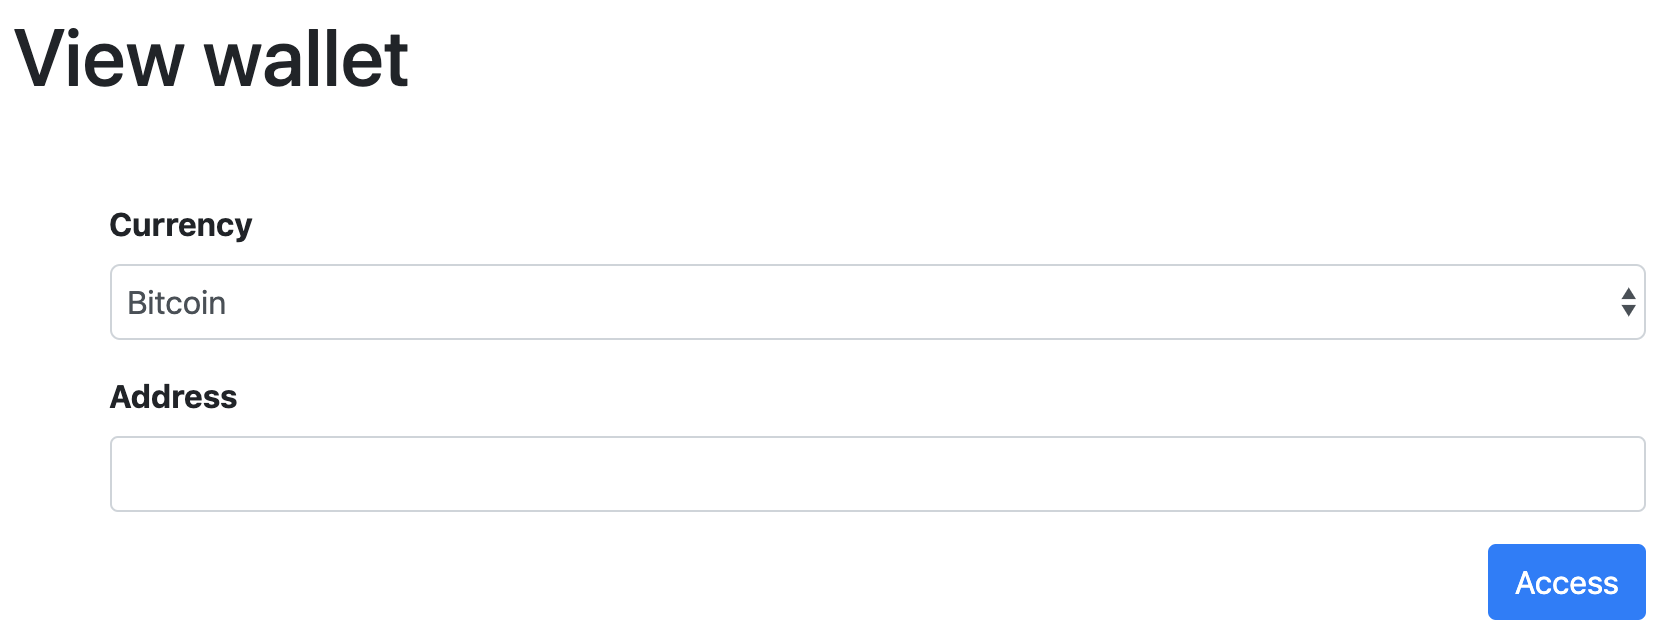
\includegraphics[width=0.7\textwidth]{assets/login.png}
    \caption{Login-like page}
    \label{5:fig:login}
\end{figure}

\newpage

\subsection{Creating or recovering wallets}

If the user doesn't have any wallet to manage yet,
they are shown an option to create a new one,
or recover one from a mnemonic phrase.
After clicking the button, they are redirected to another page
with a simple form:

\begin{figure}[ht]
    \centering
    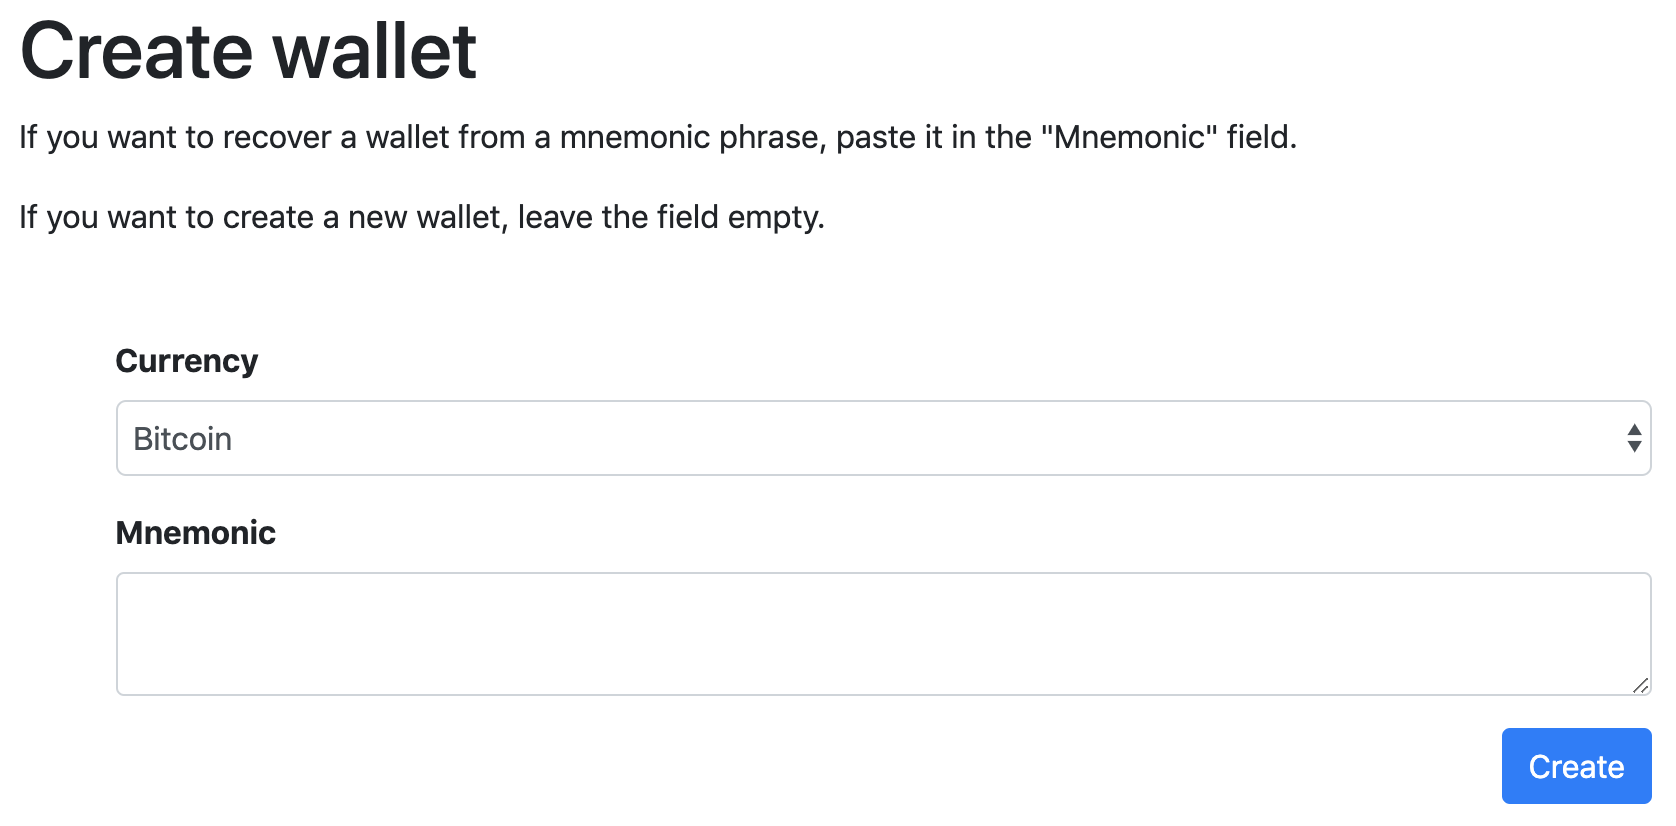
\includegraphics[width=0.7\textwidth]{assets/create-wallet.png}
    \caption{Creating a new wallet}
    \label{5:fig:create-wallet}
\end{figure}

After a successful creation of a wallet, the user is presented
with its private key and mnemonic phrase.
It's crucial to save them at this point,
because this is the last time such information will be available
(for security reasons it is not saved anywhere in the system).

\begin{figure}[ht]
    \centering
    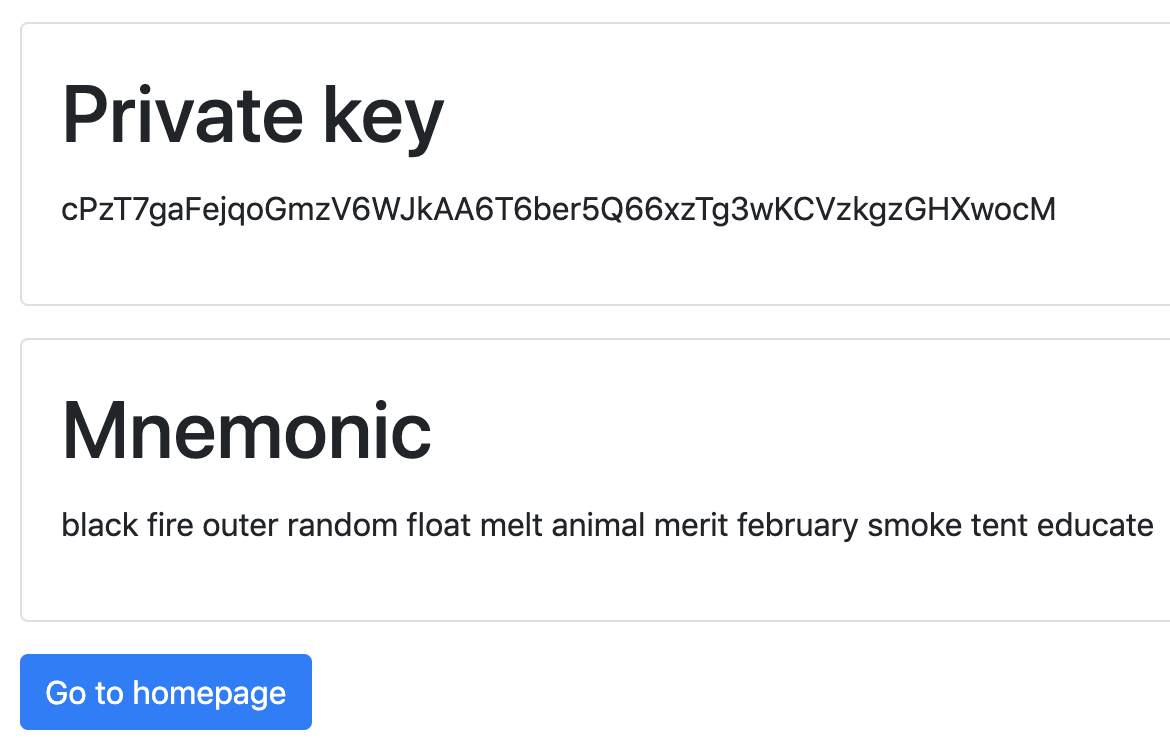
\includegraphics[width=0.7\textwidth]{assets/wallet-created.png}
    \caption{Wallet successfully created}
    \label{5:fig:wallet-created}
\end{figure}

After saving secret information, the user has an option
to be redirected to homepage in context of the newly created wallet,
as if they accessed it by its address.

\newpage

\subsection{Viewing wallets}

When using site in context of a selected address,
the user is presented with a balance over time chart and a short summary
of the funds available,
along with an option to make a transfer.

\begin{figure}[ht]
    \centering
    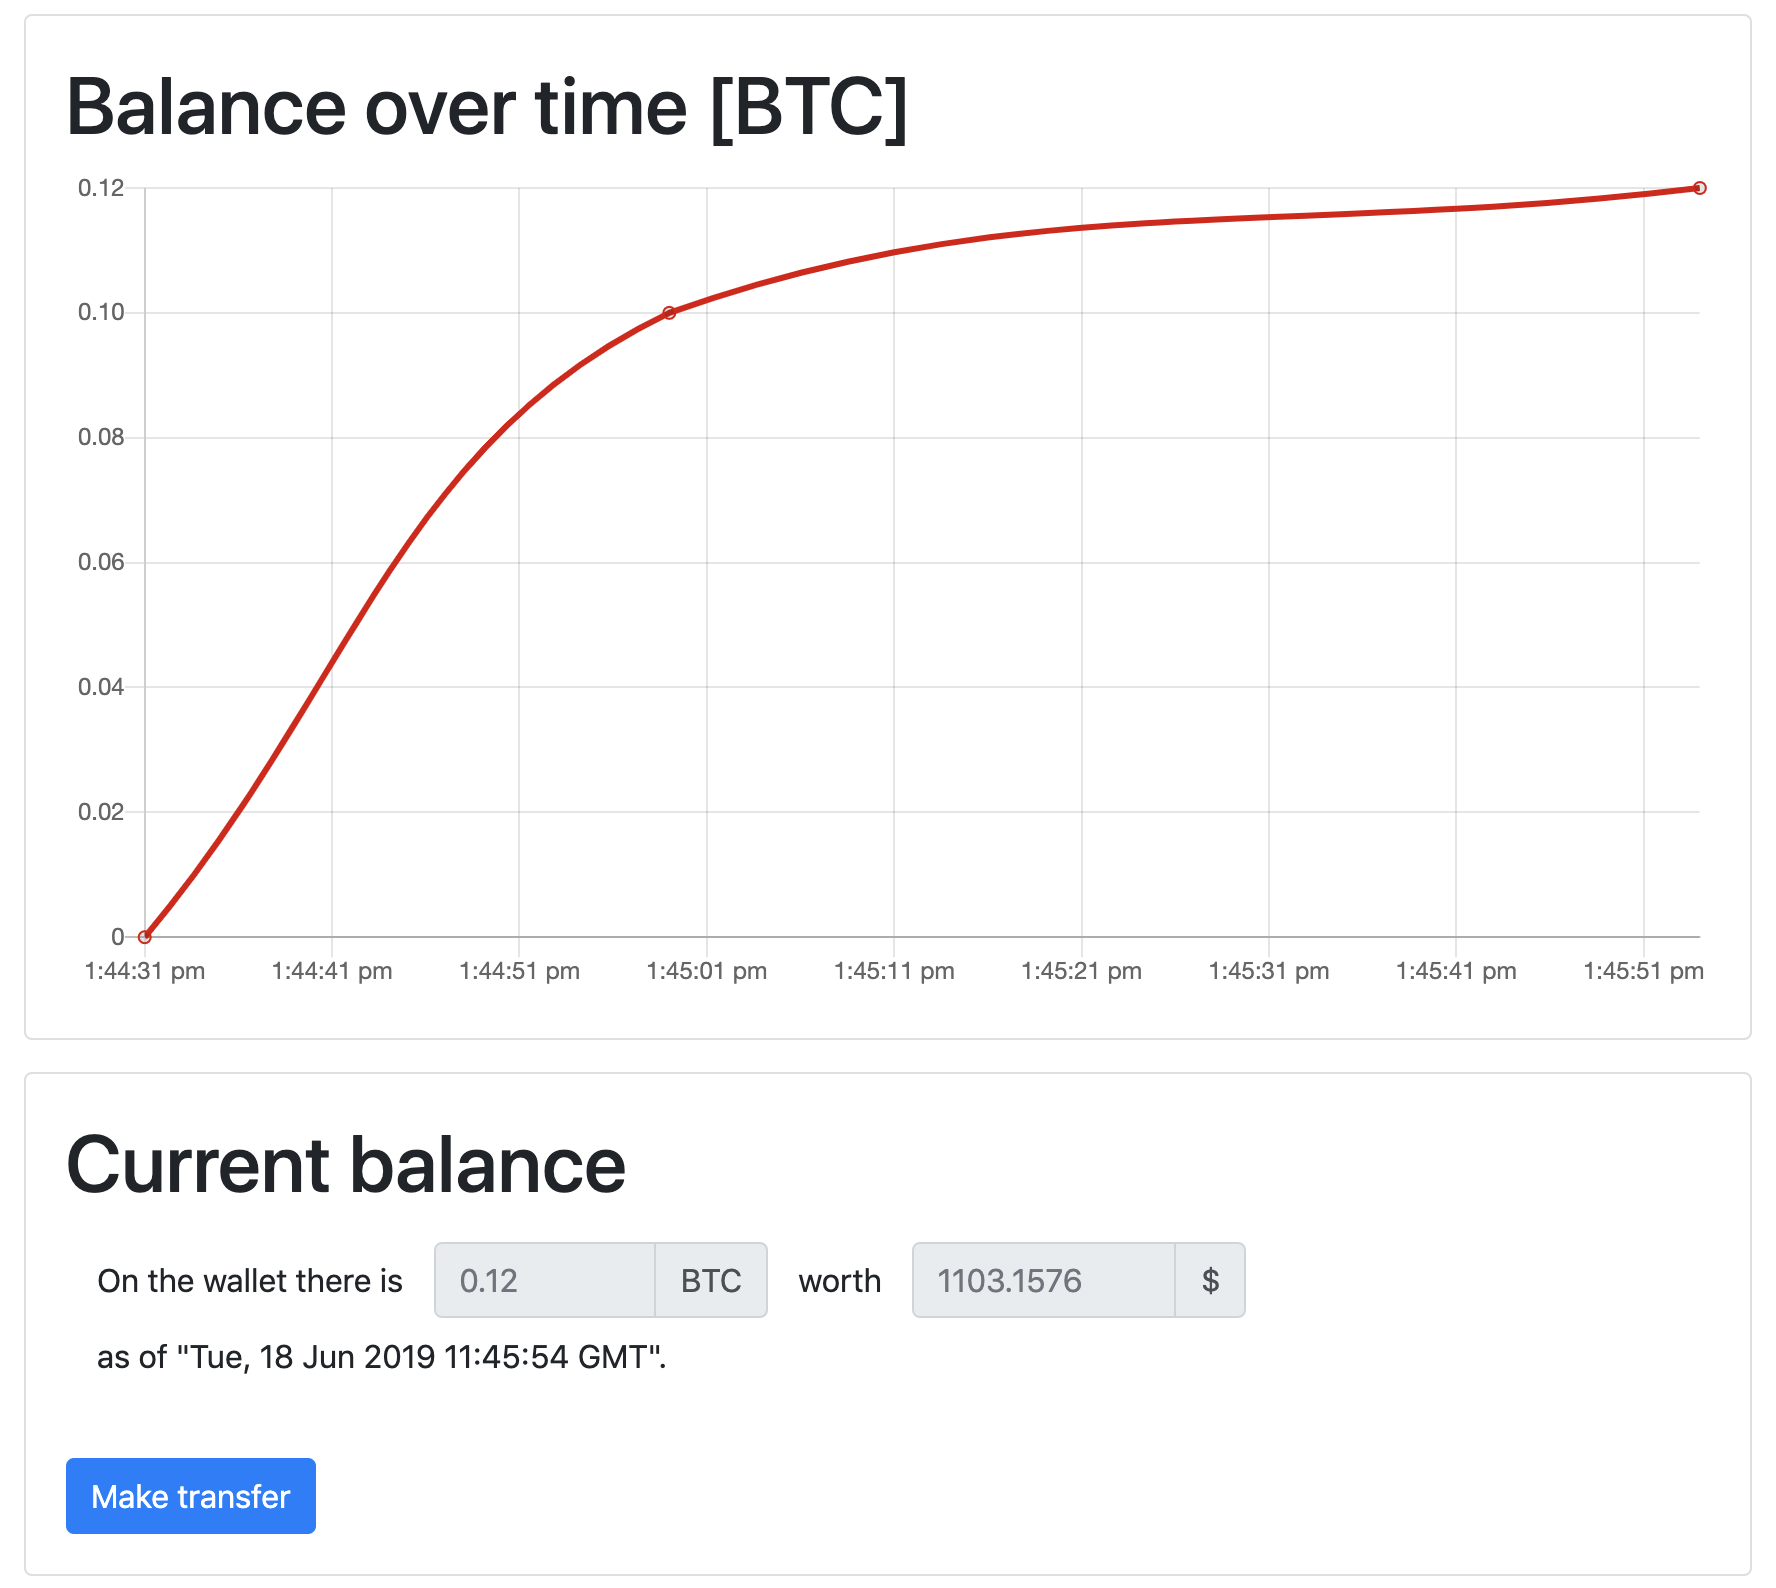
\includegraphics[width=0.7\textwidth]{assets/homepage.png}
    \caption{Homepage of a selected address}
    \label{5:fig:homepage}
\end{figure}

Below, on the same page, there is a similar chart
presenting value of the user's assets in dollars over time,
as it doesn't have to be correlated with the balance itself,
and a table providing a more detailed insight into various useful data.

During this entire time,
on all pages that current user can interact with,
they are presented with the wallet context (currency and address)
on the navigation bar.
If they wish to exit it,
the appropriate button is available in the upper-right cornet,
which is slightly similar to a logout on most websites.

\begin{figure}[ht]
    \centering
    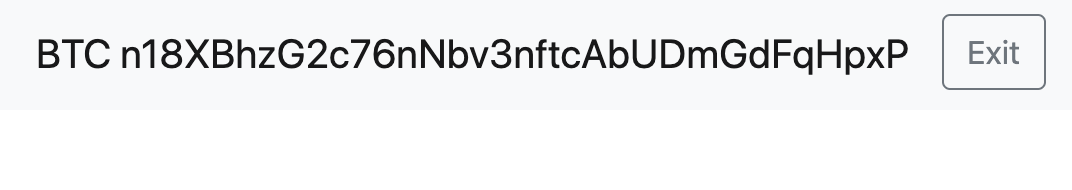
\includegraphics[width=\textwidth]{assets/logout.png}
    \caption{Wallet context}
    \label{5:fig:logout}
\end{figure}

\subsection{Making transfers}

In order to make a transfer,
the user ought to click the button described above.
After that action, they are redirected to transfers page
with a form to fill.
Desired number of recipients should be set accordingly,
and user wallet's private key must be provided for authorization.
It will be used only for this one transfer,
and will not be saved anywhere for security.
Appropriate amounts to send to their respective addresses
are to be filled in below.

\begin{figure}[ht]
    \centering
    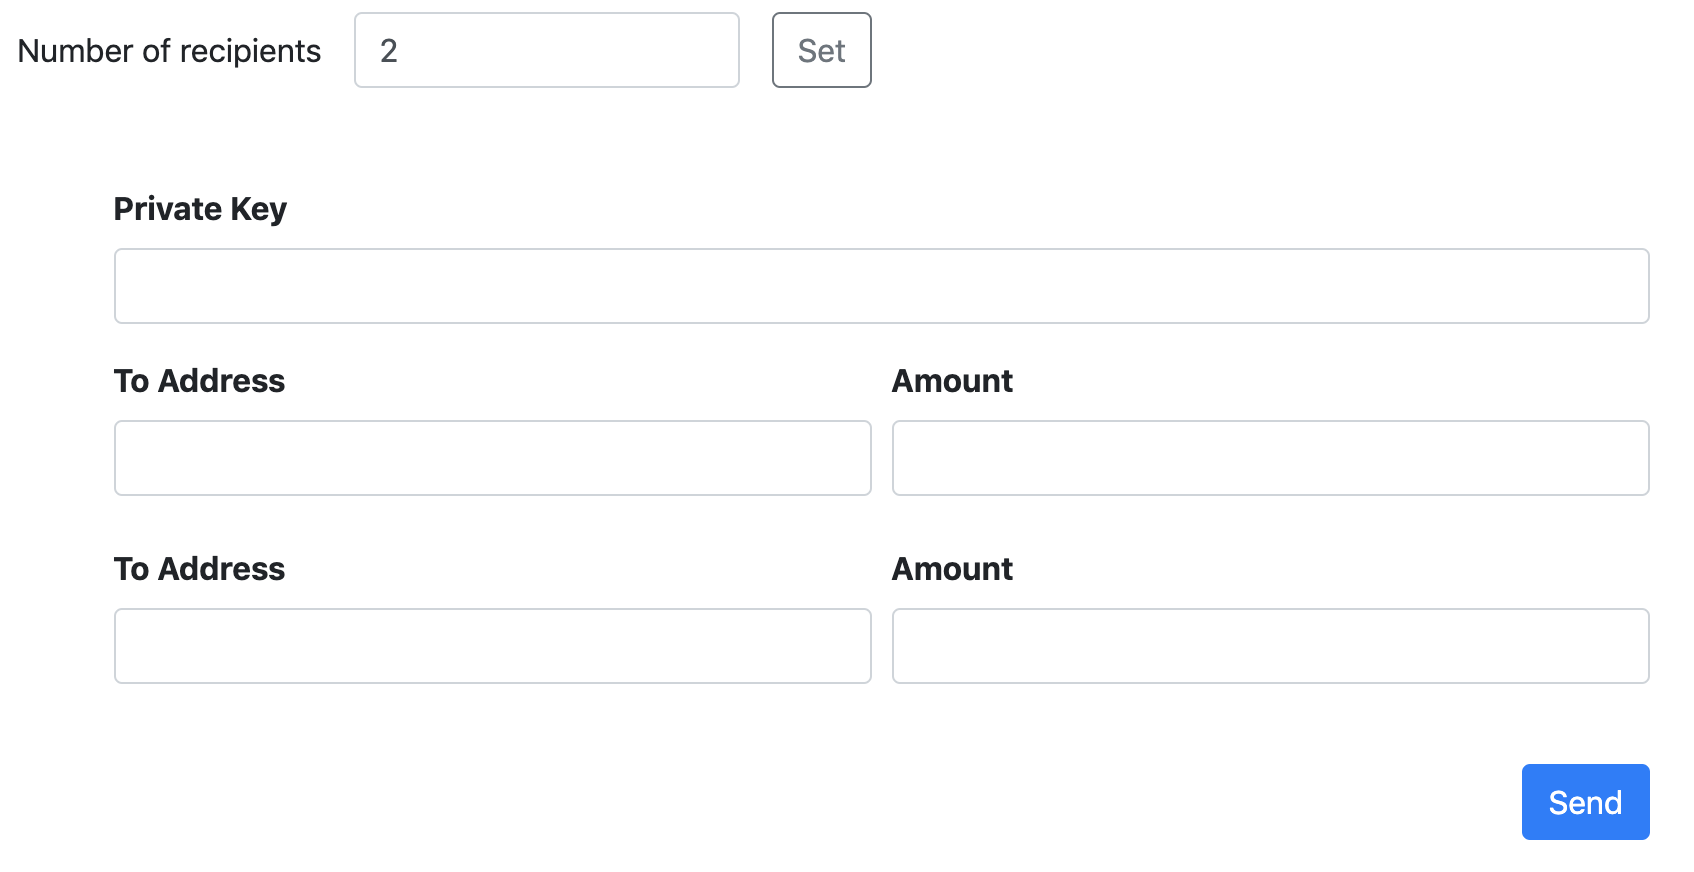
\includegraphics[width=0.7\textwidth]{assets/transfers.png}
    \caption{Transfer}
    \label{5:fig:transfers}
\end{figure}

After a successful transfer, the user will be redirected to the homepage
and provided with transaction IDs saved in the database
(only one in Bitcoin, or $n$ in case of Ethereum,
$n$ being the number of recipients).
These can be used to check transaction statuses
(e.g. numbers of confirmations)
using online blockchain explorers.

\chapter{For programmers}

The primary programming language used in the project is Python.
It was chosen because of its conciseness,
a vast array of open source third-party tools available,
such as libraries and frameworks,
and support for multiple programming paradigms,
such as imperative and object-oriented,
with functional and declarative elements.

The source code was kept in the Git \cite{git} version control system
and written using PyCharm \cite{pycharm} tool by JetBrains
on an educational license,
which can be too heavy for a small project,
but provides excellent support for code navigation and refactoring
in larger ones.

\section{Library}

\subsection{Structure}

The library consists of two major classes,
named \texttt{Bitcoin} and \texttt{Ethereum}.
They provide a unified interface for performing operations
on respective blockchains by exposing the following methods:
\begin{itemize}
    \item \texttt{create\_wallet},
    \item \texttt{get\_balance},
    \item \texttt{send\_money},
\end{itemize}
which should be self-descriptive.

There is also a class that provides an abstraction over the networking details,
which are pretty much the same in both blockchains,
as was described before.
The class is called \texttt{RpcProxy} and upon being instantiated with an URL
to an appropriate network node,
is passed to \texttt{Bitcoin} or \texttt{Ethereum} by dependency injection \cite{di}.
This allows for significant code reuse between respective currencies' classes.

\subsection{Tools} \label{6:lib:tools}

The following third-party dependencies were used to provide the library's functionality:
\begin{itemize}
    \item \texttt{pywallet} -- a library used for creating both Bitcoin and Ethereum wallets,
    chosen because of its universality,
    \item \texttt{eth-account} -- a collection of Ehtereum-specific utilities,
    used mostly for signing transactions with private keys
    (in Bitcoin this was done by the node itself),
    \item \texttt{requests} -- a tool used for making HTTP requests,
    offering a minimalistic interface better than its equivalents from the standard library;
    one of the most widely used Python libraries and a de facto standard in the industry.
\end{itemize}

For development, a unit testing framework \texttt{pytest} was also used,
providing a clean, declarative style interface superior to the standard library.
This one is not required for the library to work, though.

To test the integration with actual cryptocurrency networks,
the nodes were run as Docker containers using the Docker Compose utility,
exposing their ports for the manual and unit tests to use.
For Bitcoin, the image used was an official implementation Bitcoin Core \cite{bitcoin-core}
available as a Docker image \texttt{ruimarinho/bitcoin-core}.
Ethereum was tested against Ganache \cite{ganache},
a tool designed specifically for such use cases,
available as a Docker image \texttt{trufflesuite/ganache-cli}.

The entire library is completely independent of the web application;
it is packaged with \texttt{setuptools} to be used as if it were an external dependency.

\section{Web Application}

\subsection{Structure}

The application consists of:

\begin{itemize}
    \item request handling functions,
    \item a module exposing the library classes dynamically by currency,
    \item a module for integration with the Coinlayer API,
    \item an ORM mapping database relations to Python objects,
    \item templates for response rendering,
    \item database migrations stored as Python modules.
\end{itemize}

\subsection{Tools}

The application was created using Flask \cite{flask}, a popular Python web framework.
It is a modular tool which does not enforce any opninionated project structure,
which was desirable due to this project not being a typical CRUD backend.
Said popularity was another major advantage,
as there is now a vast array of guides and answered questions on the web.

The ORM and toolkit used for database operations is SQLAlchemy \cite{sa},
also one of the most popular Python tools of its category.
It allows for easy query construction and integrates seamlessly with Flask
thanks to the \texttt{flask-sqlalchemy} plugin.
Another plugin was \texttt{flask-migrate},
used to generate and apply database migrations with Alembic \cite{alembic}.

Web forms were created with the help of WTForms \cite{wtforms}
and its respective plugin \texttt{flask-wtf}.
This tool makes generating HTML easier, and it comes with built-in
input validation.

The \texttt{requests} library described
in \ref{6:lib:tools} was used to fetch cryptocurrency prices
from the Coinlayer API.

PostgreSQL \cite{postgres} was chosen as a database for the project,
due to popularity and its useful features.
For development, it was set up as a Docker container
along with testnet nodes and ran with Docker Compose.

HTML responses were generated with Jinja2 templating engine,
which is bundled with Flask as a sensible default option.
For styling and responsiveness Bootstrap \cite{bootstrap} CSS \cite{css} framework was used,
chosen because of popularity, ease of use and good looking design.

Last but not least, charts for viewing balances and values over time
were generated in JavaScript,
with the help of the Chart.js \cite{chartjs} library.

\chapter{Summary}

In the last chapter we shall consider some possible uses of the project
and its potential for further development.

First and foremost, the application could be used by individual users
who invest in cryptocurrencies for management of their personal wallets.
The unified interface would provide a comprehensive overview
of digital assets across different blockchains.
To get there, the project would have to be deployed on a publicly available domain,
along with a backend of several network nodes for different blockchains.
Proper configuration of such service is likely a non-trivial task,
but it has already been done by similar solutions,
e.g. the ones discussed in chapter \ref{3}.

Some other improvements in this scenario could be:
\begin{itemize}
    \item Support for more cryptocurrencies
    (many of them are based on Bitcoin or Ethereum,
    so it should not require any major changes).
    \item A more personalizable user interface,
    for instance providing an overview of all wallets
    of a given user on one screen
    (this would likely require storing user information in the database).
    \item Exchanging cryptocurrencies
    (likely requiring some legal approval).
\end{itemize}

As can be seen above, adapting the project for common use
would require some work.
There is however another scenario, for which the project could
be suitable in its current form without a need for significant modifications
-- usage by development teams working in blockchain-related projects,
such as trading platforms for instance.

Development and testing of such projects often requires dealing
with cryptocurrency wallets and making real transactions.
A simple, self-hosted tool such as this one could be quite helpful
in the process.
Managing all desired cryptocurrencies through a unified interface,
with no unnecessary clutter (like user accounts) would likely
provide a convenient way of collaboration
between members of a team.

\newpage

Additional features that would make the project better
for such use are for example:
\begin{itemize}
    \item Support for more cryptocurrencies (same as in first scenario).
    \item A more detailed insight into the blockchains,
    e.g. tracing desired transactions.
\end{itemize}

To conclude, I believe that the project shows potential for further evolution,
although development teams might be a better target group for it
than casual users.
Either way, there are many factors to consider
and many features possibly worth adding.
A core foundation that can be built upon is there,
and fulfills the requirements set at the beginning of the thesis.

Working on this project has been a valuable learning experience,
allowing me to familiarize myself with technicalities of the blockchain technology and practise designing functional user interfaces.
The ever-changing world of cryptocurrencies had seemed difficult
to grasp at times, however in the end proved to be
both a remarkable application of technology
and a promising path for further study.


%%%%% BIBLIOGRAFIA

\input{references.bbl}

\end{document}
